 \documentclass[luatex,onecolumn,showpacs,aps,preprint,prb,amsfonts,amsmath,amssymb,floatfix,groupedaddress, longbibliography]{revtex4-2} 
%\documentclass[a4paper]{article}
	\def\papertitle{Lattice dielectric properties of rutile \ce{TiO2}: \\
 First-principles anharmonic self-consistent phonon study}
	\def\authors{Tomohito Amano }
	\def\journal{}
	\def\doi{}

%%%% START preamble.tex
\usepackage[includeheadfoot,top=20mm, bottom=20mm, footskip=2.5cm]{geometry}

% Typography
\usepackage[T1]{fontenc}
\usepackage{times}
%\usepackage{mathptmx} % math also in times font
\usepackage{amssymb,amsmath}
\usepackage{microtype}
\usepackage[utf8]{inputenc}

% Misc
\usepackage{graphicx}
\usepackage[hidelinks]{hyperref} %textopdfstring from pandoc
\usepackage{soul} % Highlight using \hl{}

% Table

\usepackage{adjustbox} % center large tables across textwidth by surrounding tabular with \begin{adjustbox}{center}
\renewcommand{\arraystretch}{1.5} % enlarge spacing between rows
\usepackage{caption} 
\captionsetup[table]{skip=10pt} % enlarge spacing between caption and table

% Section styles

\usepackage{titlesec}
\titleformat{\section}{\normalfont\large}{\makebox[0pt][r]{\bf \thesection.\hspace{4mm}}}{0em}{\bfseries}
\titleformat{\subsection}{\normalfont}{\makebox[0pt][r]{\bf \thesubsection.\hspace{4mm}}}{0em}{\bfseries}
\titlespacing{\subsection}{0em}{1em}{-0.3em} % left before after

% Paragraph styles

\setlength{\parskip}{0.6\baselineskip}%
\setlength{\parindent}{0pt}%

% Quotation styles

\usepackage{framed}
\let\oldquote=\quote
\let\endoldquote=\endquote
\renewenvironment{quote}{\begin{fquote}\advance\leftmargini -2.4em\begin{oldquote}}{\end{oldquote}\end{fquote}}

\usepackage{xcolor}
\newenvironment{fquote}
  {\def\FrameCommand{
	\fboxsep=0.6em % box to text padding
	\fcolorbox{black}{white}}%
	% the "2" can be changed to make the box smaller
    \MakeFramed {\advance\hsize-2\width \FrameRestore}
    \begin{minipage}{\linewidth}
  }
  {\end{minipage}\endMakeFramed}

% Table styles

\let\oldtabular=\tabular
\let\endoldtabular=\endtabular
\renewenvironment{tabular}[1]{\begin{adjustbox}{center}\begin{oldtabular}{#1}}{\end{oldtabular}\end{adjustbox}}


% Shortcuts

%% Let textbf be both, bold and italic
%\DeclareTextFontCommand{\textbf}{\bfseries\em}

%% Add RC and AR to the left of a paragraph
%\def\RC{\makebox[0pt][r]{\bf RC:\hspace{4mm}}}
%\def\AR{\makebox[0pt][r]{AR:\hspace{4mm}}}

%% Define that \RC and \AR should start and format the whole paragraph 
\usepackage{suffix}
\long\def\RC#1\par{\makebox[0pt][r]{\bf RC:\hspace{4mm}}\textbf{\textit{#1}}\par} %\RC
\WithSuffix\long\def\RC*#1\par{\textbf{\textit{#1}}\par} %\RC*
% \long\def\AR#1\par{\makebox[0pt][r]{AR:\hspace{10pt}}\textit{#1}\par} %\AR
\long\def\AR#1\par{\makebox[0pt][r]{AR:\hspace{10pt}}#1\par} %\AR
\WithSuffix\long\def\AR*#1\par{\textit{#1}\par} %\AR*

%%%
%DIF PREAMBLE EXTENSION ADDED BY LATEXDIFF
%DIF UNDERLINE PREAMBLE %DIF PREAMBLE
\RequirePackage[normalem]{ulem} %DIF PREAMBLE
\RequirePackage{color}\definecolor{RED}{rgb}{1,0,0}\definecolor{BLUE}{rgb}{0,0,1} %DIF PREAMBLE
\providecommand{\DIFadd}[1]{{\protect\color{blue}\uwave{#1}}} %DIF PREAMBLE
\providecommand{\DIFdel}[1]{{\protect\color{red}\sout{#1}}}                      %DIF PREAMBLE
%DIF SAFE PREAMBLE %DIF PREAMBLE
\providecommand{\DIFaddbegin}{} %DIF PREAMBLE
\providecommand{\DIFaddend}{} %DIF PREAMBLE
\providecommand{\DIFdelbegin}{} %DIF PREAMBLE
\providecommand{\DIFdelend}{} %DIF PREAMBLE
%DIF FLOATSAFE PREAMBLE %DIF PREAMBLE
\providecommand{\DIFaddFL}[1]{\DIFadd{#1}} %DIF PREAMBLE
\providecommand{\DIFdelFL}[1]{\DIFdel{#1}} %DIF PREAMBLE
\providecommand{\DIFaddbeginFL}{} %DIF PREAMBLE
\providecommand{\DIFaddendFL}{} %DIF PREAMBLE
\providecommand{\DIFdelbeginFL}{} %DIF PREAMBLE
\providecommand{\DIFdelendFL}{} %DIF PREAMBLE
%DIF END PREAMBLE EXTENSION ADDED BY LATEXDIFF

% Define title defaults if not defined by user
\providecommand{\lettertitle}{Author Response to Reviews of}
\providecommand{\papertitle}{Title}
\providecommand{\authors}{Authors}
% \providecommand{\journal}{Journal}
% \providecommand{\doi}{--}

% % preamble

% This is for template only !!
\usepackage{lipsum}

%\usepackage{floatrow}
\usepackage{siunitx}
\usepackage{color}
\usepackage{hhline}
\usepackage{mathrsfs}
\usepackage[dvipdfmx]{graphicx}
\usepackage{adjustbox}
\usepackage{dcolumn}
\usepackage{bm}% bold math
\usepackage{multirow}
\usepackage{booktabs}
\usepackage{afterpage}
\usepackage{amsmath}
\usepackage{ulem}
\usepackage{physics}

% https://mathlandscape.com/latex-underline/
\usepackage{ulem}

\usepackage{here} % force figures Here.

\usepackage[inline]{asymptote}

\usepackage[compat=1.1.0]{tikz-feynhand} % feynman diagram
% subcaption http://www.yamamo10.jp/yamamoto/comp/latex/make_doc/insert_fig/index.php#SUBCAP
% https://oku.edu.mie-u.ac.jp/tex/mod/forum/discuss.php?d=1024
% https://atatat.hatenablog.com/entry/cloud_latex18_subcaption
\usepackage{caption}
\usepackage[subrefformat=parens]{subcaption}
%\usepackage{floatrow}
%\usepackage[export]{adjustbox}

% http://www.yamamo10.jp/yamamoto/comp/latex/make_doc/chemistry/index.php
\usepackage[version=4]{mhchem}

% for tikz 
\usepackage{tikz, pgf, pgfplots, pgfplotstable}
\usepackage{tikz-3dplot}
\usetikzlibrary{math,calc}
\pgfplotsset{compat = newest}
\usepgfplotslibrary{groupplots} % LATEX and plain TEX
\pgfplotsset{compat = newest}

\pgfplotsset{
   table/search path={figures/self_energy, figures/tdos, figures/diel_func, figures/band},
}

\graphicspath{{figures/self_energy, figures/tdos, figures/diel_func, figures/band}}

% https://tikz.dev/library-external
% crisさんおすすめ
% \usetikzlibrary{external}
% \tikzexternalize % activate!

\usepackage{multirow}


\usepackage[subpreambles=true,sort=true]{standalone}

%https://uec.medit.link/latex/table.html#:~:text=%E3%82%BB%E3%83%AB%E3%81%AE%E7%B5%90%E5%90%88,%E3%82%92%E8%AA%AD%E3%81%BF%E8%BE%BC%E3%82%80%E5%BF%85%E8%A6%81%E3%81%8C%E3%81%82%E3%82%8B%E3%80%82

% \usepackage[no-math,haranoaji,deluxe]{luatexja-preset}
%https://mizunashi-mana.github.io/blog/posts/2021/12/migrate-to-luatexja/

\newcommand{\red}[1]{\textcolor{red}{#1}}
\newcommand{\blue}[1]{\textcolor{blue}{#1}}
\arraycolsep=0.0em
\setlength{\abovecaptionskip}{0mm}
\setlength{\belowcaptionskip}{0mm}
\usepackage{caption} 
\captionsetup[table]{skip=8pt}
\captionsetup[figure]{skip=4pt}
%\setlength{\MidlineHeight}{2pt}


\usepackage{comment}
%\usepackage{natbib}

\usepackage[colorlinks=true,citecolor=blue,linkcolor=blue,urlcolor=blue]{hyperref}
\usepackage{cleveref}
\crefname{equation}{Eq.}{Eq.}% {環境名}{単数形}{複数形} \crefで引くときの表示
\crefname{figure}{Fig.}{Fig.}% {環境名}{単数形}{複数形} \crefで引くときの表示
\crefname{table}{Table}{Table}% {環境名}{単数形}{複数形} \crefで引くときの表示
\crefname{section}{Sec.}{Sec.}% {環境名}{単数形}{複数形} \crefで引くときの表示
\crefname{appendix}{Appendix}{Appendix}% {環境名}{単数形}{複数形} \Crefで引くときの表示


\Crefname{equation}{Equation}{Equation}% {環境名}{単数形}{複数形} \Crefで引くときの表示
\Crefname{figure}{Figure}{Figure}% {環境名}{単数形}{複数形} \Crefで引くときの表示
\Crefname{table}{Table}{Table}% {環境名}{単数形}{複数形} \Crefで引くときの表示
\Crefname{section}{Section}{Section}% {環境名}{単数形}{複数形} \Crefで引くときの表示
\Crefname{appendix}{Appendix}{Appendix}% {環境名}{単数形}{複数形} \Crefで引くときの表示



\usepackage{threeparttable} %https://qiita.com/kumamupooh/items/38795811fc6b934a950d
% bookmark
% \usepackage{xurl}
% \hypersetup{unicode,bookmarksnumbered=true,hidelinks,final}


\newcommand{\ph}{\phantom{0}}

\renewcommand{\topfraction}{1.0}
\renewcommand{\bottomfraction}{1.0}
\renewcommand{\dbltopfraction}{1.0}
\renewcommand{\textfraction}{0.1}
\renewcommand{\floatpagefraction}{0.9}
\renewcommand{\dblfloatpagefraction}{0.9}




% others ...
\usepackage{siunitx}
\usepackage{standalone}
\usepackage{mhchem}
% \usepackage[colorlinks=true,citecolor=blue,linkcolor=blue,urlcolor=blue]{hyperref}

\usepackage{graphicx}

% 
\renewcommand{\thefigure}{A\arabic{figure}}
\renewcommand{\thetable}{A\arabic{table}}
% \setcounter{figure}{0}
% \setcounter{table}{0}


\usepackage{cleveref}
\crefname{figure}{Fig.}{Fig.}% {環境名}{単数形}{複数形} \crefで引くときの表示
\crefname{table}{Table}{Table}% {環境名}{単数形}{複数形} \crefで引くときの表示


% biblatex
% \usepackage[%
% backend=bibtex,
% style=phys,%
% articletitle=false,biblabel=brackets,%
% chaptertitle=false,pageranges=false,%
% ]{biblatex}
% \addbibresource{../references/tio2_ref.bib}


\usepackage{comment}	% required for `\comment' (yatex added)
\begin{document}


% Make title
{\Large\bf \lettertitle}\\[1em]
{\huge \papertitle}\\[1em]
{\authors}\\
% {\it \journal, }\texttt{doi:\doi}\\
\hrule

% Legend
\hfill {\bfseries RC:} \textbf{\textit{Reviewer Comment}},\(\quad\) AR: \emph{Author Response}, \(\quad\square\) Manuscript text

\section{the First Referee}

\subsection{General comment}

\RC This work studies the anharmonic lattice dynamics of rutile \ce{TiO2} using the newly developed selfconsistent phonon + bubble (SCPH+B) theory. The SCPH+B incorporates the third-order anharmonic bubble self-energy into the original SCPH theory. The anharmonic phonon frequencies and linewidths of the Gamma point optical phonons produced by the SCPH+B are improved significantly with respect to those by harmonic calculations or conventional perturbative approach. Now the theoretical optical properties are in much better agreement with reported experimental measurements. Results obtained by two different functionals, LDA and $\mathrm{r}^2$SCAN, are compared and discussed.
Experimentally observed but unidentified peaks of the dielectric function are attributed to the two-phonon emission process, which is included by the frequency-dependent bubble term. This work is novel and comprehensive. Therefore, I recommend that it should be published in Physical Review B once the authors address the following minor points.

\AR We sincerely appreciate the referee’s supportive and insightful comments on our manuscript. We believe this manuscript will interest many researchers as it discusses the dielectric properties of rutile \ce{TiO2} with a detailed analysis of its anharmonic phonons. Following the suggestions of the referee, we have amended the manuscript appropriately. We provided the point-by-point responses to the referee’s comments/questions below:

\subsection{\#1}

\RC I understand the current method improves the phonon frequencies and linewidths significantly. How about the renormalization effect on eigenvectors? Take the phonon modes shown in Fig. 1 for example. How different are the eigenvectors obtained by harmonic calculations, SCPH, and SCPH+B, respectively?

\AR  We thank the reviewer for pointing out the renormalization effect on phonon eigenvectors. First, in the current calculation, phonon eigenvectors change in SCPH, while SCPH+B does not cause changes from SCPH in eigenvectors because we do not include off-diagonal components of the bubble self-energy. The SCPH eigenvectors of the $E_{u}$ modes differ slightly from harmonic approximation in their relative magnitude of \ce{Ti} and \ce{O} displacements, but at an almost negligible level. 

Renormalization of phonon eigenvectors is important when an imaginary phonon exists, but the influence is limited because rutile \ce{TiO2} has no imaginary phonon. As can be seen from Eq. (3), eigenvectors are necessary to calculate the dielectric function, so the eigenvectors also need to be calculated accurately as well as the eigenvalues. However, in the rutile \ce{TiO2} case, the difference in the eigenvectors between the harmonic approximation and SCPH+B makes almost no difference in the dielectric function either. 

Since we did not mention the renormalization effect of phonon eigenvectors in the original submitted version of the manuscript, we have added the following sentence in the dielectric function section:

\begin{quote}
On the other hand, in the $E^{2}_{\mathrm{u}}$ and $E^{3}_{\mathrm{u}}$ phonons, the two \ce{Ti} atoms move in opposite directions, so the mode oscillator strength is much smaller. \DIFadd{The renormalization of phonon eigenvectors by SCPH is negligible, and it is the phonon frequencies and self-energies that affect the calculation results of dielectric properties.} The SCPH+B calculations agree remarkably...
\end{quote}

\begin{comment}
 The cat in the box is \DIFdelbegin \DIFdel{dead}\DIFdelend \DIFaddbegin \DIFadd{alive}\DIFaddend .
 \begin{align}
  E &= mc^2 \\
  m\cdot \DIFdelbegin \DIFdel{a=F}\DIFdelend \DIFaddbegin \DIFadd{v=p}\DIFaddend .
 \end{align}
\end{comment}



\subsection{\#2}

\RC In Table III, the harmonic $B_{1u}^{1}$ frequency by $\mathrm{r}^2$SCAN agrees with the experiment much better than the anharmonic frequencies, no matter which method is used. This is also seen in the same optical branch along Gamma-M and Gamma-X in Fig. 3(a). Any idea why anharmonic frequencies agree with experiments worse than harmonic ones?

\AR  We sincerely appreciate the referee’s perceptive remarks about the discrepancy between our SCPH+B calculation and experiments regarding the phonon bands. There seem to be different factors for this discrepancy between LDA and $\mathrm{r}^2$SCAN. 

 As for LDA, because the Gr\"{u}neisen parameter of this mode is positive, underestimating the lattice parameter leads to an overestimation of the frequency. From this point of view, it is natural that SCPH+B overestimates the frequency in the LDA. When calculated using the experimental lattice constant at $\SI{300}{\kelvin}$, the SCPH+B calculation gives a frequency of $\SI{124}{\per\cm}$ at $\SI{300}{\kelvin}$, which better agrees with the experiment. 

In the $\mathrm{r}^2$SCAN functional, however, the Gr\"{u}neisen constant cannot explain the overestimation of the frequencies because the lattice constant is larger than the experimental value. We think the inability to accurately describe the $B_{\mathrm{1u}}^{1}$ branch is likely due to the $\mathrm{r}^2$SCAN functional rather than our anharmonic phonon calculations, because the potential energy surface of the $B_{\mathrm{1u}}^{1}$ phonon is better explained by the anharmonic calculation than the harmonic approximation, as in \cref{fig:b1u}.

\begin{figure}[htb]
% \input{pes/merged/pes.tex} % 2つ
\centering
% \includestandalone[mode=image]{figures/pes/A2u/pes_a2u} %A2uのみ (オリジナル)
\includestandalone[mode=image]{../figures/pes/B1u/input_R2SCAN2/pes_b1u_standalone} %A2uのみ (x軸の修正版)
\caption{Frozen phonon potential (blue) of $B^1_{\mathrm{1u}}$ mode with $x$ axis being the normal coordinate of $B^1_{\mathrm{1u}}$ phonon.}
\label{fig:b1u}
\end{figure}

To discuss the dependence on the functional, we also performed SCPH+B calculations using the PBEsol functional. \cref{table:lattice_constant_pbesol} shows the optimized lattice parameters, and \cref{fig:pbesolband} shows the band dispersion with SCPH+B. As can be seen here, despite PBEsol having a smaller lattice constant than $\mathrm{r}^2$SCAN, the frequency of the $B_{\mathrm{1u}}^{1}$ mode is $\SI{121}{\per\cm}$, which is smaller than that of $\mathrm{r}^2$SCAN and reproduces the experimental value~\cite{traylor1971Lattice} well.

\begin{table}[t] % lattice_constant::PBEsol
\centering
\caption{Calculated lattice constants with LDA, $\mathrm{r}^2$SCAN and PBEsol.}
\includestandalone[mode=tex]{../table_standalone/lattice_constant_RC2} % lattice constants
\label{table:lattice_constant_pbesol}
\end{table}%

\begin{figure}[tb] % PBEsolのバンド図
\centering
\includestandalone[mode=image]{../figures/band/pbesol_standalone} %PBEsol vs r2SCANのバンド図
%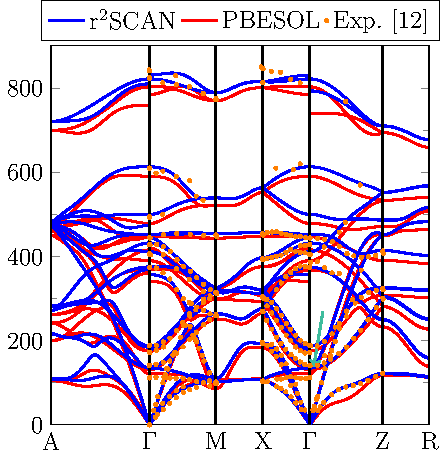
\includegraphics{pbesol_vs_r2scan.pdf}
\caption{The SCPH+B band structure with $\mathrm{r}^2$SCAN (red) and PBEsol (blue) functional. The green arrow indicates the $B_{\mathrm{1u}}^{1}$ mode, which is overestimated in the $\mathrm{r}^2$SCAN functional. }
\label{fig:pbesolband}
\end{figure}

% reported the differencesではなくて,reported differencesが正解?
For rutile \ce{TiO2}, several previous studies reported differences in the results originating from functionals and pseudopotentials~\cite{montanari2002Lattice,shojaee2009Firstprinciples,mitev2010Soft}. The choice of the correct functionals and pseudopotentials is still an open question. The PBEsol functional describes the $B_{\mathrm{1u}}^{1}$ modes well, but the overall phonon frequency agreement is better with $\mathrm{r}^2$SCAN. In the present study, we have focused on the lattice dielectric properties, and have used the $\mathrm{r}^2$SCAN functional to better describe the lattice constants and IR-active phonon modes. To make this point clearer, we have revised the manuscript as follows.

\begin{quote}
\DIFadd{Overall,} the combination of the $\mathrm{r}^2$SCAN functional and the SCPH+B calculation agrees well with the experimental data \DIFadd{except for the lowest optical phonon mode ($B_{\mathrm{1u}}$), which is known to be sensitive to the choice of functionals.}
\end{quote}

The results and discussion of the PBEsol functional results have been added in the section 2-E and the appendix B.

\subsection{\#3}

\RC In Fig. 3(b) and the first paragraph of Page 7, the authors indicated a generally good agreement between LDA and $\mathrm{r}^2$SCAN phonon dispersions and LDA’s overestimation of A$_{2u}$ frequency due to its underestimation of volume (optimized at static zero pressure). I think it may be a better idea to compare LDA and $\mathrm{r}^2$SCAN phonon dispersions at the same volume, say the experimental value, disregarding the calculated pressure. If that is the case, is LDA still good to use for vibrational properties calculations of \ce{TiO2} and related materials?

\AR  We thank the referee for the insightful suggestion. To confirm this point, we carried out SCPH+B calculations with LDA using the lattice constants obtained by the experiment and the $\mathrm{r}^2$SCAN. When we used the lattice constant of $\mathrm{r}^2$SCAN, which is greater than the experimental value, $\mathrm{A}_{2u}$ became unstable. If we used the experimental lattice constant, the frequency of the $A_{\mathrm{2u}}$ phonon is $\SI{146}{\per\cm}$, which is $15 \%$ smaller than the experimental value. 

Our additional calculations confirm that the behavior of the lattice constant-sensitive $\mathrm{A}_{2u}$ modes, noted in previous harmonic phonon studies, is also seen at the level of anharmonic phonon calculations. Even if experimental lattice constants were used, the LDA would not correctly reproduce the frequencies of the $\mathrm{A}_{2u}$ modes, demonstrating the effectiveness of $\mathrm{r}^2$SCAN.

To better clarify the sensitivity of the $\mathrm{A}_{2u}$ mode to the lattice constants, we added the following sentence to the manuscript:

\begin{quote}
The underestimation of the lattice constants of LDA may cause the overestimation of the $A_{\mathrm{2u}}$ phonon, as the $A_{\mathrm{2u}}$ phonon is sensitive to lattice constants. \DIFadd{To clarify this point, we have performed the SCPH+B calculation with LDA using the experimental lattice constants. The resultant frequency of the $A_{\mathrm{2u}}$ phonon was $\SI{146}{\per\cm}$ , which underestimatesthe experimental value by $15\%$. This result shows that the $A_{\mathrm{2u}}$ mode is sensitive to the lattice constant even at the level of anharmonic phonon calculations.} For the LO phonons, the LDA results overestimate the ...
\end{quote}


\subsection{\#4}

\RC In Table IV, except for the TO E$_{u}^{1}$ mode, the 4ph contribution to the rest of the phonon modes’ linewidth by the SCPH+B is not as significant as the bubble contribution, yet non-negligible. Whereas in the abstract, it is stated, “We show that the four-phonon scattering process contributes as much as the third-order anharmonic term to phonon linewidths.” Perhaps this statement can be improved.

\AR  We thank the referee for pointing this out. We agree that the $4$-ph contribution is as large as the bubble contribution only in TO E$_{u}^{1}$ and $A_{\mathrm{2u}}$ phonons, and that the original manuscript was incorrect. We have amended the abstract as follows:

\begin{quote}
We show that the four-phonon scattering process contributes as much as the third-order anharmonic term to phonon linewidths \DIFadd{of some phonon modes}.
\end{quote}


 % references
% \bibliographystyle{apsrev4-2}
% \bibliography{references/tio2_ref.bib}
%\printbibliography

\newpage
\section{The Second Referee}

\subsection{General Comment}

\RC In this paper, the authors calculated the lattice dielectric function of \ce{TiO2} by the anharmonic self-consistent phonon approach. The SCPH+
bubble (SCPH+B) theory proposed by [T. Tadano et al. Phys. Rev. Lett. 129, 185901 (2022)] is used, which includes the bubble phonon scattering. The importance of phonon anharmonic effect in the calculation of dielectric function is illustrated by comparing with experimental results. For typical phonon modes, the contribution of four-phonon scattering process to the phonon linewidth is not negligible. Anharmonic phonon properties and related issues, such as dielectric function are meaningful topics. The novelty of this paper mainly lies in the study and discussion of the necessity of phonon anharmonic correction of dielectric function. Before considering publication in PRB, the authors need to consider the following comments.

\AR We sincerely appreciate the referee’s insightful comments on our manuscript. We believe this manuscript will interest many researchers as it discusses the dielectric properties of rutile \ce{TiO2} with a detailed analysis of its anharmonic phonons. Following the suggestions of the referee, we have amended the manuscript appropriately. We provided the point-by-point responses to the referee’s comments/questions below:

\subsection{\#1}

\RC The temperature-dependent static dielectric constant in the $x$ direction obtained by the SCPH+B method is in good agreement with the experimental data, while the difference in the $z$ direction is very large (Fig. 5), which obviously should not be attributed to the bubble scattering. The authors need to discuss this issue.

\AR We sincerely appreciate the referee's perceptive comment on the temperature-dependent static dielectric constant in the $z$ direction. Our calculation underestimates the static dielectric constant $\epsilon_0^z$ in the low temperature region. According to Eq. (3), the underestimation of $\epsilon_0^z$ is due to the overestimation of the frequency of the $A_{\mathrm{2u}}$ phonon. %The result indicates that our calculation overestimates the zero-point vibration in the $A_{\mathrm{2u}}$ mode. 

%Actually, \cref{fig_phi4} shows the large mode dependent contribution to the loop self-energy of $A_{\mathrm{2u}}$ phonon at $\SI{0}{\kelvin}$. ( $V(q=A_{2u},-q=A_{2u},q',-q')\frac{\hbar}{2\omega_{q'}}$ ) 

To see whether this large deviation comes from our SCPH+B calculation, we performed the SCPH+B calculation using the PBEsol functional, which yielded the $\mathrm{A}_{2u}$ frequency of $\SI{162}{\per\cm}$ at $\SI{300}{\kelvin}$, close to that of $\mathrm{r}^2$SCAN. \cref{fig:temp_a2u} shows the temperature dependence of the frequency of the $\mathrm{A}_{2u}$ phonon, where PBEsol is in good agreement with experiment at low temperatures, while r2SCAN overestimates the frequency at low temperatures. As a result, calculated $\epsilon_0^z$ with PBEsol is in good agreement with experimental data in \cref{fig:temp_diel}. From this calculation, we consider that the underestimation of $\epsilon_0^z$ by the $\mathrm{r}^2$SCAN functional is more likely to be due to the functional than to our anharmonic phonon calculations.

% As shown in Fig. 4, our IFCs model reproduces the DFT calculations well, and the cause may lie in the DFT calculations.

 % \begin{figure}[htb]
 % % \input{pes/merged/pes.tex} % 2つ
 % \centering
 % % \includestandalone[mode=image]{figures/pes/A2u/pes_a2u} %A2uのみ (オリジナル)
 % 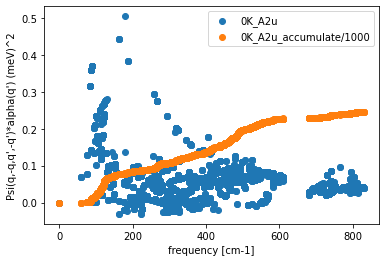
\includegraphics[width=8.6cm]{phi4.png}
 % \caption{mode dependent contribution to the loop self-energy of $A_{\mathrm{2u}}$ phonon at $\SI{0}{\kelvin}$. ( $V(q=A_{2u},-q=A_{2u},q',-q')\frac{\hbar}{2\omega_{q'}}$)}
 % \label{fig_phi4}
 % \end{figure}


\begin{figure}[tb] % 
\centering
\includestandalone[mode=image]{../figures/temp_dep_a2u/temp_dep_a2u_RC} %PBEsol vs r2SCANのバンド図
%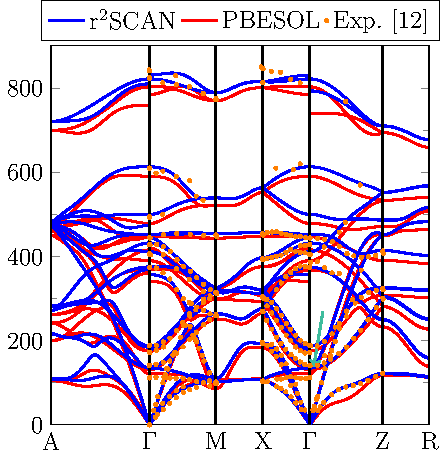
\includegraphics{pbesol_vs_r2scan.pdf}
\caption{The temperature dependence of $\mathrm{A}_{2u}$ phonon of the $\mathrm{r}^2$SCAN (blue) and PBEsol (orange) functional togather with experimental data (red). The red triangles represent the experimental values~\cite{parker1961static}} 
\label{fig:temp_a2u}
\end{figure}

\begin{figure}[tb] % 
\centering
\includestandalone[mode=image]{../figures/temp_dep_diel/temp_dep_diel_final_RC2} %PBEsol vs r2SCAN 誘電定数
%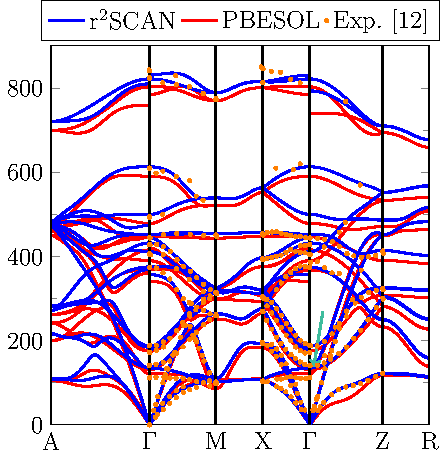
\includegraphics{pbesol_vs_r2scan.pdf}
\caption{The temperature dependence of the static dielectric constant $\epsilon_0^z$ with the $\mathrm{r}^2$SCAN (blue) and PBEsol (orange) functional. The red triangles represent the experimental values~\cite{parker1961static}} 
\label{fig:temp_diel}
\end{figure}

Since we did not include the explanation for the deviation, we added the following sentence.

 \begin{quote}
The SCPH+B calculation well reproduced experimental values for $\epsilon^0_x$. For $\epsilon^{0}_z$, on the other hand, the tendency to increase is reproduced, but the value at $T=0$ is $169$, which is only $70\%$ of the experimental value. \DIFadd{In fact, the frequency of the $A_{\mathrm{2u}}$ mode at $T=0$ is $\SI{167}{\per\cm}$ in the SCPH+B calculation, compared to $\SI{140}{\per\cm}$ for the experimental value, which indicates that the zero-point vibration is very large. This could be improved by using more acurate functionals like hybrid functionals.}
\end{quote}

Also, the results and discussion of the PBEsol functional results have been added in section 2-E and appendix B.


\subsection{\#2}

\RC Although the SCPH+B is significant to correct the phonon frequency and phonon width for specific phonon modes, some typical modes, such as $E^{3}_{\mathrm{u}}$ ($\SI{26.5}{\per\cm}$) and $A_{\mathrm{2u}}$ ($\SI{16.2}{\per\cm}$) listed in Table IV, have a larger deviation from experimental results ($\SI{43.9}{\per\cm}$ and $\SI{46.4}{\per\cm}$) compared with non-SC results ($\SI{41.4}{\per\cm}$ and $\SI{30.4}{\per\cm}$). Do phonon scattering processes beyond the bubble scattering play a major role?

\AR  We sincerely appreciate the referee’s insightful question on the discrepancy in linewidths in the LO phonons. We agree that the agreement between SCPH+B and the experiment is not good for the LO $E^{3}_{\mathrm{u}}$ and $A_{\mathrm{2u}}$ phonons. The LO $E^{3}_{\mathrm{u}}$ and $A_{\mathrm{2u}}$ modes have high frequencies at about $\SI{800}{\per\cm}$, and the number of phonons contributing to these self-energies is not large. It is, therefore, reasonable that the bubble diagram is smaller for these LO modes than for TO modes.

Generally, higher-order contribution is more important in the high-frequency region, such as LO $E^{3}_{\mathrm{u}}$ and $A^{2}_{\mathrm{u}}$ phonons. We may get better results by including higher-order diagrams, but higher-order calculations are difficult at this stage due to computational costs. %However, the evaluation of higher-order diagrams is currently difficult from a computational point of view.

In addition, the non-SC result of LO $E^{3}_{\mathrm{u}}$ and $A_{\mathrm{2u}}$ phonons coincidentally matches the experimental values, because the non-SC reflectivity shown in Fig.4 is well below the experimental values. The reflectivity of theoretical calculations is usually larger than that of experiments, as there are no impurities, surfaces, and interfaces between a substrate and a thin film that can occur in experiments.

%It should also be mentioned again that the values given in Table IV are the result of fitting with the FPSQ model: the non-SC results for E3u and $\mathrm{A}_{2u}$ are in good agreement with the model, but the reflectivity (Figure 6) significantly underestimates the experimental values. We consider that the non-SC results do not correctly describe reality, 

We added the following sentence about the role of higher-order diagrams to the linewidth section.

\begin{quote}
 It indicates that the calculation of linewidth requires accurate determination of phonon frequencies, including anharmonicity, as pointed out by Fu et al. \DIFadd{Discrepancies are observed in the $E^{1}_{\mathrm{u}}$ and $A_{\mathrm{2u}}$ TO modes with relatively high frequencies, which could be improved by incorporating higher-order diagrams.} We also found that self-energies ...
\end{quote}



\subsection{\#3}

\RC The contribution of the four-phonon scattering process to phonon linewidth is only significant for $E_{\mathrm{u}^1}$ and $A_{\mathrm{2u}}$ modes. For other modes, however, the contribution of four-phonon scattering is much lower than the three-phonon scattering. Therefore, the statement of "We show that the four-phonon scattering process contributes as much as the third-order anharmonic term to phonon linewidths" in the abstract should be rewritten.

\AR  We thank the referee for pointing this out. We agree that the $4$-ph contribution is as large as the bubble contribution only in TO $E_{\mathrm{u}}^{1}$ and $A_{\mathrm{2u}}$ phonons, and that the original manuscript was incorrect. We have amended the abstract as follows:

\begin{quote}
 We show that the four-phonon scattering process contributes as much as the third-order anharmonic term to phonon linewidths \DIFadd{of some phonon modes}.
\end{quote}

\subsection{\#4}

\RC “Figure 3b demonstrates a good agreement between between LDA and $\mathrm{r}^2$SCAN throughout the Brillouin zone.”The word "between" is repeated.

\AR  We thank the referee for pointing out the error. We have fixed it.


 % references
% \bibliographystyle{apsrev4-2}
% \bibliography{references/tio2_ref.bib}
%\printbibliography

\newpage
\section{The Third Referee}

\subsection{General Comment}

\RC Amano and co-workers report a first principles study of the dielectric properties of \ce{TiO2} using an anharmonic description of the lattice
dynamics. Specifically, they use a self-consistent phonon theory including third and fourth-order terms. With this, they discuss temperature-dependent phonon frequencies, linewidths, and derived quantities, which are in general in good agreement with experiment. They are also able to assign a number of previously unidentified peaks of the dielectric function to two-phonon processes. 
Rutile \ce{TiO2} is a scientifically and technologically interesting material, and the authors use state-of-the-art methods to describe its dielectric behavior. They clearly show that anharmonic lattice dynamics is essential for an accurate description of this compound. I would like the authors to consider:

\AR We sincerely appreciate the referee’s supportive and insightful comments on our manuscript. We believe this manuscript will interest many researchers as it discusses the dielectric properties of rutile \ce{TiO2} with a detailed analysis of its anharmonic phonons. Following the suggestions of the referee, we have amended the manuscript appropriately. We provided the point-by-point responses to the referee’s comments/questions below:

\subsection{\#1}

\RC In Fig. 3(a), it looks like the harmonic (red) curve agrees better with experiment (orange dots). This is particularly clear with the lowest energy optical mode at the Gamma point. The authors instead write in the text: "The combination of the $\mathrm{r}^2$SCAN functional and the SCPH+B calculation agrees well with the experimental data", seemingly ignoring the better agreement with harmonic calculations for some modes? Along the same lines, from Table III a mixed picture emerges, where agreement with experiment is best for different combinations of theory depending on the mode. Can the authors comment on these points?

\AR  We sincerely appreciate the referee’s perceptive remarks about the discrepancy between our SCPH+B calculation and the experiment regarding the phonon bands. For the lowest optical phonon branch ($\mathrm{B}_{1u}$), there seem to be different factors for this discrepancy between LDA and $\mathrm{r}^2$SCAN. 

 As for LDA, because the Gr\"{u}neisen parameter of this mode is positive, underestimating the lattice parameter leads to an overestimation of the frequency. From this point of view, it is natural that SCPH+B overestimates the frequency in the LDA. When calculated using the experimental lattice constant at $\SI{300}{\kelvin}$, the SCPH+B calculation gives a frequency of $\SI{124}{\per\cm}$ at $\SI{300}{\kelvin}$, which better agrees with the experiment. 

In the $\mathrm{r}^2$SCAN functional, however, the Gr\"{u}neisen constant cannot explain the overestimation of the frequencies because the lattice constant is larger than the experimental value. We think the inability to accurately describe the $B_{\mathrm{1u}}^{1}$ branch is likely due to the $\mathrm{r}^2$SCAN functional rather than our anharmonic phonon calculations, because the potential energy surface of the $B_{\mathrm{1u}}^{1}$ phonon is better explained by the anharmonic calculation than the harmonic approximation, as in \cref{fig:b1u2}.

\begin{figure}[htb]
% \input{pes/merged/pes.tex} % 2つ
\centering
% \includestandalone[mode=image]{figures/pes/A2u/pes_a2u} %A2uのみ (オリジナル)
\includestandalone[mode=image]{../figures/pes/B1u/input_R2SCAN2/pes_b1u_standalone} %A2uのみ (x軸の修正版)
\caption{Frozen phonon potential (blue) of $B_{\mathrm{1u}}$ mode with $x$ axis being the normal coordinate of $B_{\mathrm{1u}}$ phonon.}
\label{fig:b1u2}
\end{figure}

To discuss the dependence on the functional, we also performed SCPH+B calculations using the PBEsol functional. \cref{table:lattice_constant_pbesol2} shows the optimized lattice parameters, and \cref{fig:pbesol2} shows the band dispersion with SCPH+B. As can be seen here, despite PBEsol having a smaller lattice constant than $\mathrm{r}^2$SCAN, the frequency of the $B_{\mathrm{1u}}^{1}$ mode is $\SI{121}{\per\cm}$, which is smaller than that of $\mathrm{r}^2$SCAN and reproduces the experimental value well.

\begin{table}[t] % lattice_constant::PBEsol
\centering
\caption{calculated lattice constants with LDA, $\mathrm{r}^2$SCAN and PBEsol.}
\includestandalone[mode=tex]{../table_standalone/lattice_constant_RC2} % lattice constants
\label{table:lattice_constant_pbesol2}
\end{table}%

\begin{figure}[tb] % PBEsolのバンド図
\centering
\includestandalone[mode=image]{../figures/band/pbesol_standalone} %PBEsol vs r2SCANのバンド図
%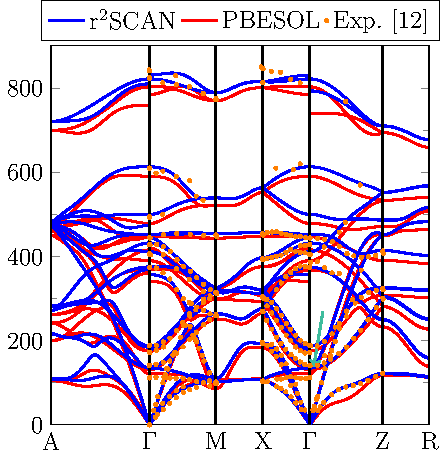
\includegraphics{pbesol_vs_r2scan.pdf}
\caption{The SCPH+B band structure with r2SCAN (red) and PBEsol (blue) functional. The green arrow indicates the $\mathrm{B}_{1u}^{1}$ mode, which is overestimated in the r2SCAN functional. }
\label{fig:pbesol2}
\end{figure}

Similarly, we agree that the best theory for each $\Gamma$-point phonon frequency is different in Table III. What is important, however, is that the combination of $\mathrm{r}^2$SCAN and SCPH+B gives an overall good description, especially for strongly anharmonic modes. More detailed comparisons on each phonon mode are difficult, as the results depend not only on anharmonic phonon calculations but also on the choice of functionals or pseudopotentials.


% reported the differencesではなくて,reported differencesが正解?
For rutile \ce{TiO2}, several previous studies reported differences in the results originating from functionals and pseudopotentials~\cite{montanari2002Lattice,shojaee2009Firstprinciples,mitev2010Soft}. The choice of the correct functionals and pseudopotentials is still an open question. In the present study, we have focused on the lattice dielectric properties, and have used the $\mathrm{r}^2$SCAN functional to better describe the lattice constants and IR-active phonon modes. To make this point clearer, we have revised the manuscript as follows.

\begin{quote}
\DIFadd{Overall}, the combination of the $\mathrm{r}^2$SCAN functional and the SCPH+B calculation agrees well with the experimental data \DIFadd{except for the lowest optical phonon mode ($B_{\mathrm{1u}}$), which is known to be sensitive to the choice of functionals.}
\end{quote}

The results and discussion of the PBEsol functional results have been added in the section 2-E and the appendix B.

\subsection{\#2}

\RC Can the authors speculate as to why the temperature dependence of $\epsilon_z$ is not well-reproduced in Fig. 5?

\AR We sincerely appreciate the referee's insightful comment on the temperature-dependent static dielectric constant in the $z$ direction. Our calculation underestimates the static dielectric constant $\epsilon_0^z$ in the low temperature region. According to Eq. (3), the underestimation of $\epsilon_0^z$ is due to the overestimation of the frequency of the $A_{\mathrm{2u}}$ phonon. % The result indicates that our calculation overestimates the zero-point vibration in the $A_{\mathrm{2u}}$ mode. 

%Actually, \cref{fig_phi4} shows the large mode dependent contribution to the loop self-energy of $A_{\mathrm{2u}}$ phonon at $\SI{0}{\kelvin}$. ( $V(q=A_{2u},-q=A_{2u},q',-q')\frac{\hbar}{2\omega_{q'}}$ ) 

To see whether this large deviation comes from our SCPH+B calculation, we performed the SCPH+B calculation using the PBEsol functional, which yielded the $A_{\mathrm{2u}}$ frequency of $\SI{162}{\per\cm}$ at $\SI{300}{\kelvin}$, close to that of $\mathrm{r}^2$SCAN. \cref{fig:temp_a2u2} shows the temperature dependence of the frequency of the $A_{\mathrm{2u}}$ phonon, where PBEsol is in good agreement with the experiment at low temperatures, while $\mathrm{r}^2$SCAN overestimates the frequency at low temperatures. As a result, calculated $\epsilon_0^z$ with PBEsol is in good agreement with the experimental data in \cref{fig:temp_diel2}. From this calculation, we consider that the underestimation of $\epsilon_0^z$ by the $\mathrm{r}^2$SCAN functional is more likely to be due to the functional than to anharmonic phonon calculations.

% As shown in Fig. 4, our IFCs model reproduces the DFT calculations well, and the cause may lie in the DFT calculations.

 % \begin{figure}[htb]
 % % \input{pes/merged/pes.tex} % 2つ
 % \centering
 % % \includestandalone[mode=image]{figures/pes/A2u/pes_a2u} %A2uのみ (オリジナル)
 % 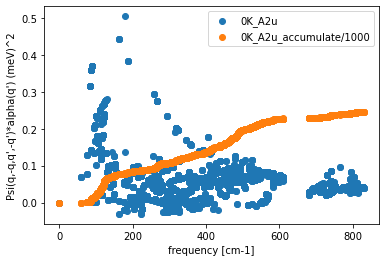
\includegraphics[width=8.6cm]{phi4.png}
 % \caption{mode dependent contribution to the loop self-energy of $A_{\mathrm{2u}}$ phonon at $\SI{0}{\kelvin}$. ( $V(q=A_{2u},-q=A_{2u},q',-q')\frac{\hbar}{2\omega_{q'}}$)}
 % \label{fig_phi4}
 % \end{figure}


\begin{figure}[tb] % 
\centering
\includestandalone[mode=image]{../figures/temp_dep_a2u/temp_dep_a2u_RC} %PBEsol vs r2SCANのバンド図
%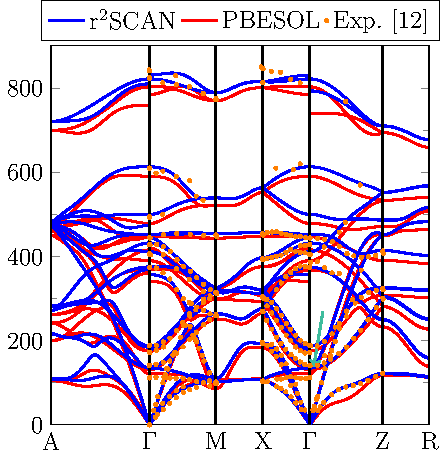
\includegraphics{pbesol_vs_r2scan.pdf}
\caption{The temperature dependence of $A_{\mathrm{2u}}$ phonon of the $\mathrm{r}^2$SCAN (blue) and PBEsol (orange) functional togather with the experimental data (red).} 
\label{fig:temp_a2u2}
\end{figure}

\begin{figure}[tb] % 
\centering
\includestandalone[mode=image]{../figures/temp_dep_diel/temp_dep_diel_final_RC2} %PBEsol vs r2SCAN 誘電定数
%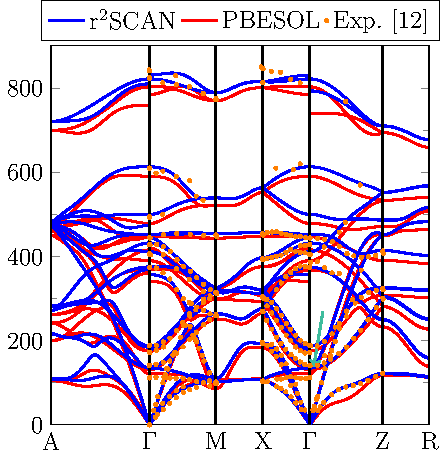
\includegraphics{pbesol_vs_r2scan.pdf}
\caption{The temperature dependence of the static dielectric constant $\epsilon_0^z$ with the $\mathrm{r}^2$SCAN (blue) and PBEsol (orange) functional. The red triangles represent the experimental values~\cite{parker1961static}.} 
\label{fig:temp_diel2}
\end{figure}



% Our calculation underestimates the static dielectric constant $\epsilon_0^z$ in low temperature. According to Eq. (3), the underestimation of $\epsilon_0^z$ is due to the overestimation of the frequency of $A_{\mathrm{2u}}$, \cref{fig_phi4} shows the large mode dependent contribution to the loop self-energy of $A_{\mathrm{2u}}$ phonon at $\SI{0}{\kelvin}$. ( $V(q=A_{2u},-q=A_{2u},q',-q')\frac{\hbar}{2\omega_{q'}}$ ) As shown in Fig. 4, our IFCs model reproduces the DFT calculations well, and the cause may lie in the DFT calculations.

% \begin{figure}[htb]
% % \input{pes/merged/pes.tex} % 2つ
% \centering
% % \includestandalone[mode=image]{figures/pes/A2u/pes_a2u} %A2uのみ (オリジナル)
% 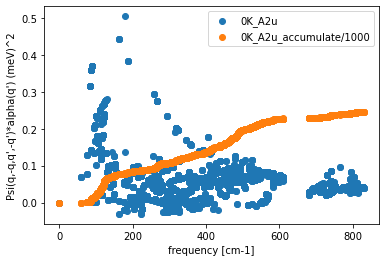
\includegraphics[width=8.6cm]{phi4.png}
% \caption{mode dependent contribution to the loop self-energy of $A_{\mathrm{2u}}$ phonon at $\SI{0}{\kelvin}$. ( $V(q=A_{2u},-q=A_{2u},q',-q')\frac{\hbar}{2\omega_{q'}}$)}
% \label{fig_phi4}
% \end{figure}

Since we did not include the explanation for the deviation, we added the following sentence.

 \begin{quote}
The SCPH+B calculation well reproduced experimental values for $\epsilon^0_x$. For $\epsilon^{0}_z$, on the other hand, the tendency to increase is reproduced, but the value at $T=0$ is $169$, which is only $70\%$ of the experimental value. \DIFadd{In fact, the frequency of the $A_{\mathrm{2u}}$ mode at $T=0$ is $\SI{167}{\per\cm}$ in the SCPH+B calculation, compared to $\SI{140}{\per\cm}$ for the experimental value, which indicates that the zero-point vibration is very large. This could be improved by using more acurate functionals like hybrid functionals.}
\end{quote}

\subsection{\#3}

\RC More generally, the authors show that four-phonon processes are important, sometimes comparable to three-phonon process. Based on this, could the authors justify stopping at four-phonon processes? What role could higher-order processes play?

\AR  We thank the reviewer for pointing out the role of higher-order diagrams. The higher order terms generally become significant in high-frequency regime since higher-order diagrams involve more phonons and contributions are more likely to appear at higher frequencies. Therefore we expect that they have minor roles in low frequency regime, where we focus in this paper. On the other hand, remaining discrepancies for $E^{3}_\mathrm{u}$ and $A_{\mathrm{2u}}$ modes, having high frequencies ($\SI{800}{\per\cm}$) may be corrected by those higher order terms.
Unfortunately, those possibilities and any numerical instabilities in the low-frequency regime are beyond our capabilities since the first-principle evaluation of terms higher than fourth for compounds is prohibitively demanding and yet unprecedented in the community.

% ここの2段落は明石さんによって上のように修正された.
% First, as regards the justification for stopping the expansion at the 4ph diagram, it should be noted that the bubble diagram is still larger in the whole frequency domain, even though the 4ph diagram is sometimes comparable to the bubble diagram for the linewidths shown in Fig. 4. Also, higher-order diagrams have not been calculated in previous studies, which pointed out the importance of the four-phonon diagram, mainly due to computational costs. 

% Secondly, as regards the role played by higher-order diagrams, higher-order contribution is more important in the high-frequency region, such as in LO $E^{3}_\mathrm{u}$ and $A_{\mathrm{2u}}$ in general. This is because higher-order diagrams involve more phonons, so contributions are more likely to appear at higher frequencies. We expect that including higher-order correction can improve the results for the lifetime of these two modes in Table IV. However, again, the calculation is difficult due to computational costs. 

We added the following sentence about the role of higher-order diagrams to the linewidth section.

\begin{quote}
 It indicates that the calculation of linewidth requires accurate determination of phonon frequencies, including anharmonicity, as pointed out by Fu et al. \DIFadd{Discrepancies are observed in the $E^{1}_{\mathrm{u}}$ and $A_{\mathrm{2u}}$ TO modes with relatively high frequencies, which could be improved by incorporating higher-order diagrams.} We also found that self-energies ...
\end{quote}

\newpage
\section{The List of changes made}

These are highlighted by red in the attached highlighted manuscript except for minor grammatical corrections.

\begin{itemize}
  \item The abstract has benn slightly modified for more accurate description.
  \item We have performed PBEsol calculations, and have added related results and discussions. (III-A,III-E,Appendix B)
  \item Figure. 4 was wrong in the original version, and we replaced it with correct one.
  \item We have performed LDA calculations using the experimental lattice constants, and the result has been added to III-B (page 6).
  \item A discussion has been given as to why the calculated and experimental values of $\epsilon_0^z$ at low temperature do not agree in III-B (page 7).
  \item We have added the discussion on a possible cause of the descrepancy of linewidth between experiments and our culculation in III-C (page 7).
  \item We have added the sentence discussing phonon eigenvectors renormalization in III-D (page 8).
  \item JSR Corporation has been added in Acknowledgement (page 11).
  \item Some minor corrections have been made to improve readability and clarity.
\end{itemize}

 % references

% ================ bibtex 
 \bibliographystyle{apsrev4-2}
 \bibliography{../references/tio2_ref.bib}
% ================

% for biblatex
% \printbibliography


\end{document}
